\chapter{Tests}
Diese Testdokumentation wurde erstellt, um die Herangehensweise, Durchführung sowie die Ergebnisse unseres Testprozesses festzuhalten. 

\section{Ziele}
Ziel unseres Testprozesses ist es garantieren zu können, dass die in diesem Projekt geschaffene Software unter den von uns festgelegten Vorraussetzungen annähernd bis vollständig fehlerfrei und mit möglichst guter Performance betrieben werden kann. Auffälligkeiten sowie nach dem Testprozess bekannte und nicht behobene Fehler sollen am Ende des Testprozesses dokumentiert sein.

\section{Rahmenbedingungen}
Grundsätzlich wurde während der Entwicklung der Anwendung stets darauf geachtet, dass die jeweils neu implementierten Features einwandfrei funktionieren und auch, dass durch die Implementierung jener Features keine der zuvor vorhandenen Teile beschädigt werden. Dennoch haben wir in unserer Projektplanung eine gesonderte Testphase geplant, bei der wir im Zeitraum von zwei Wochen alle nötigen Schritte abschließen möchten, um die von uns erstellte Anwendung ausgiebig zu testen. In dieser zweiwöchigen Testphase soll der Testprozess vollständig abgeschlossen werden. Alle einzelnen Tests von Fron-End sowie Back-End wurden dabei jeweils in der selben Testumgebung durchgeführt.

\section{Teststrategie}
Um unser Testziel zu erreichen greifen wir auf verschiedene Testmethoden zurück. Da die Testphase sowohl durch einen kurzen Zeitraum, als auch die Anzahl der Tester eingeschränkt ist, müssen wir diese Ressourcen bestmöglich nutzen. Nach längeren Diskussionen innerhalb des Entwicklungsteams haben wir uns dazu entschlossen, auf eine Kombination von automatisierten Unit-Tests, manuellen System- und UI-Tests, sowie Last-Test zu setzen. Auf diese Weise decken wir beim Testen nicht nur funktionale sondern auch qualitative Anforderungen der Software ab.

Welche Methodik bei den einzelnen Teilen der Anwendung verwendet wurde wird in der folgenden Tabelle \ref{testarten_software} dargestellt.

\begin{table}[]
	\begin{tabular}{|l|l|}
		\cline{1-2}
		\textbf{Testobjekt} & \textbf{Art des Testens} \\ \cline{1-2}
		Front-End           & \begin{tabular}[c]{@{}l@{}}Unit-Tests,\\ Manuelle Tests\end{tabular} \\ \cline{1-2}
		Back-End            & \begin{tabular}[c]{@{}l@{}}Unit-Tests.\\ Manuelle Tests\end{tabular} \\ \cline{1-2}
		Gesamtsystem        & \begin{tabular}[c]{@{}l@{}}Manuelle Tests,\\ Last-Tests\end{tabular} \\ \cline{1-2}
	\end{tabular}
\caption{Testarten der unterschiedlichen Softwareteile}
\label{testarten_software}
\end{table}

Trotz dessen, dass wir eine eigene Testphase geplant haben, ist es uns wichtig über den gesamten Entwicklungsprozess der Software für eine stets einwandfrei lauffähige Anwendung zu sorgen. Dies entspricht nicht nur unserem agilen Softwareentwicklungsprozess nach Scrum, sondern erleichtert auch die gemeinsame Arbeit durch mehrere Entwickler jeweils an Front-End sowie Back-End. Um dies gewährleisten zu können, haben wir abseits der Testphase jedes neu implementierte Feature sowie die Auswirkungen der Implementierung auf den Rest der Anwendung manuell getestet.

\section{Testen des Front-Ends}

\subsection{Unit-Tests}
Bei unserem Front-End sind wir zu dem Schluss gekommen, dass ein automatisiertes Testen nur bedingt sinnvoll ist. Ein großer Teil der Implementierungen dort bezieht sich rein auf die Darstellung der vom Back-End erhaltenen Daten im Webbrowser, oder um das Beschaffen und Versenden eben dieser Daten. Ein automatiertes Testen der Weboberfläche ist dabei überproportional aufwändig und in unserem Falle in den meisten Fällen nicht sinnvoll, da es sich vor allem um statische Inhalte oder um Video- beziehungsweise Bildinhalte handelt. Außerdem muss beim Testen einer Weboberfläche auf Faktoren wie Browserkompatibilität geachtet werden, was durch manuelles Testen besser umsetzbar ist. Nichts desto trotz wurde für jede Komponente des Front-Ends ein eigener Unit-Test erstellt, der die vollständige Erzeugung eben dieser Komponente simuliert und testet. Dabei werden für die Komponente erforderliche Abhängigkeiten durch Mock-Objekte ersetzt, um ein unabhängiges Testen zu ermöglichen.

Standardgemäß verwenden wir beim automatisierten Testen unseres Angular-Front-Ends das Testframework Karma. Dieses ist bereits beim Erzeugen eines neuen Angular-Projektes per Angular-\acs{CLI} integriert und vorkonfiguriert. 

\subsubsection{Ausführen der Unit-Tests}
Nachdem das Projekt korrekt auf die in \ref{chapter_installation} Dargestellte Art und Weise installiert wurde und lauffähig ist, können die automatisierten Tests durch das Aufrufen eines Konsolenbefehls gestartet werden. Dazu muss im Projektordner ein Terminal geöffnet werden und der Befehl \glqq{}ng test\grqq ausgeführt werden.

\subsubsection{Ergebnisse der Unit-Tests}

\begin{figure}[ht]
	\flushright
	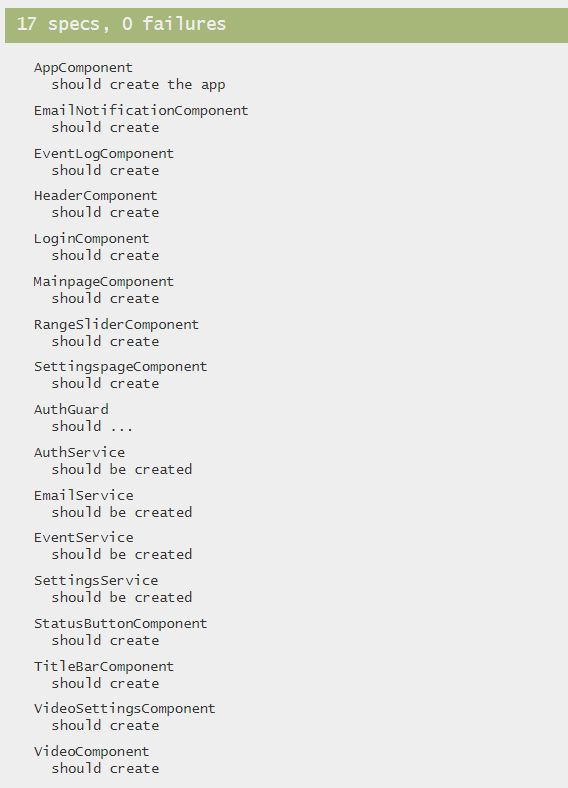
\includegraphics[]{content/pictures/ErgebnisseAutomatisierteTestsFrontend.jpg}
	\caption{Ergebnisse der automatisierten Front-End-Tests}
	\label{fig:ergebnisse_autom_tests_frontend}
\end{figure}


\subsection{Manuelle Tests}
\label{subsection_manuelle_tests}
Beim manuellen testen handelt es sich um einen Testprozess, bei dem der Tester ohne die Verwendung von Automatisierungstools vorgeht. Dabei können durch die systematische Verwendung der Software und das Nutzen von Diagnosetools oft Fehler aufgedeckt werden, die etwa bei Unit-Tests häufig nicht gefunden werden. Insbesondere Benutzeroberflächen können auf diese Weise unkompliziert getestet werden.

Im folgenden wird tabellarisch festgehalten, welche Aktionen getestet wurden und von welcher Ausgangssituation aus getestet wurde. Alle Tests wurden in den beiden Browsern Google Chrome (64-Bit Version 71.0.3578.98 Offizieller Build) und Mozilla Firefox (64-Bit Version 63.0.1 Offizieller Build) auf einem mit Windows 10 betriebenem Laptop mit einer Auflösung von 1920x1080 durchgeführt. 

\subsubsection{Ergebnisse der Manuellen Tests}
Vorraussetzung für alle Tests ist selbsterklärend, dass Front-End sowie Back-End korrekt installiert und gestartet sind. Zudem sind alle Einstellungen sinnvoll gewählt. Das bedeutet beispielsweise, dass ein funktionierender MJPEG-Stream hinterlegt ist. Es sind außerdem fünf beliebige Clips mit allen nötigen Werten korrekt gespeichert sowie abrufbar. Es sind auch zwei gespeichert.

Folgende Einstellungen waren bei den folgenden manuellen Tests vorhanden:

\begin{longtable}{| p{.2\textwidth} | p{.6\textwidth} |}
	\hline
	\textbf{Einstellung} & \textbf{Wert} \\ \hline

	sensitivity & 0.0 \\ \hline
		
	brightness & 0.5 \\ \hline
		
	contrast & 1.0 \\ \hline
		
	global\_notify & true \\ \hline
		
	log\_enabled & true \\ \hline
		
	streamaddress & https://webcam1.lpl.org/axis-cgi/mjpg/video.cgi \\ \hline
		
	cliplength & 10 \\ \hline
		
	max\_logs & 20 \\ \hline
		
	max\_storagee & 1024 \\ \hline
	
\caption{Eingestellte Werte vor jedem manuellen Test}
\label{tab:eingestellte_werte_vor_tests}
\end{longtable}

Erklärung zur nachfolgenden Tabelle \ref{tab:manuelle_front_end_tests} der manuellen Front-End-Tests:\newline

Bedeutung der Spalte C*: Der Test wurde in der zuvor genannten Version von Google Chrome erfolgreich durchgeführt.\newline

Bedeutung der Spalte F*: Der Test wurde in der zuvor genannten Version von Mozilla Firefox erfolgreich durchgeführt.

\newcounter{TestNumber}
\begin{longtable}{| p{.02\textwidth} | p{.08\textwidth} | p{.25\textwidth} | p{.25\textwidth} | p{.25\textwidth} | p{.025\textwidth} | p{.025\textwidth} |}
	\hline
	
	\textbf{\#} & \textbf{Kom-po-nen-te} & \textbf{Vorraussetz-ungen} & \textbf{Aktion} & \textbf{Erwartetes Ergebnis} & \textbf{C*} & \textbf{F*} \\ \hline
	
	\stepcounter{TestNumber}\arabic{TestNumber} & Login & Der Anwender befindet sich auf der Login-Seite und ist demnach nicht eingeloggt. & Der Anwender gibt beim Einloggen den richtigen Usernamen (user) und das richtige Passwort (geheim) ein. & Der Anwender wird auf die Hauptseite der Anwendung weitergeleitet und ist	korrekt eingeloggt. & X & X \\ \hline
	
	\stepcounter{TestNumber}\arabic{TestNumber} & Login & Der Anwender befindet sich auf der Login-Seite und ist demnach nicht
	eingeloggt. & Der Anwender gibt beim
	Einloggen einen falschen Usernamen (Verwendet: test) und das richtige Passwort (geheim) ein. & Rechts neben dem Login-Button erscheint eine Nachricht (Login failed) in roter Schrift. & X & X \\ \hline
	
	\stepcounter{TestNumber}\arabic{TestNumber} & Login & Der Anwender befindet sich auf der Login-Seite und ist demnach nicht
	eingeloggt. Das Back-End ist nicht erreichbar. & Der Anwender versucht sich einzuloggen. & Rechts neben dem Login-Button erscheint eine Nachricht (Login failed) in roter Schrift. & X & X \\ \hline
	
	\stepcounter{TestNumber}\arabic{TestNumber} & Login & Der Anwender befindet sich auf der Login-Seite und ist demnach nicht eingeloggt. & Der Anwender gibt beim
	Einloggen den richtigen Usernamen (user) und ein falsches Passwort ein. (Verwendet: test) & Rechts neben dem Login-Button  erscheint eine Nachricht (Login failed) in roter Schrift. & X & X \\ \hline
	
	\stepcounter{TestNumber}\arabic{TestNumber} & Login & Der Anwender befindet sich auf der Login-Seite	und ist demnach nicht
	eingeloggt. & Der Anwender gibt beim Einloggen sowohl einen falschen Usernamen (Verwendet: test1) als auch ein falsches Passwort (Verwendet: test2) ein. & Rechts neben dem Login-Button erscheint eine Nachricht (Login failed) in roter Schrift. & X & X \\ \hline
	
	\stepcounter{TestNumber}\arabic{TestNumber} & Login & Der Anwender befindet sich auf der Login-Seite und ist demnach nicht eingeloggt. & Der Anwender gibt beim Einloggen einen falschen Usernamen (Verwendet: test) und das richtige Passwort (geheim) ein. & Zwischen dem Absenden der Logindaten und dem Empfangen einer Antwort durch das Back-End wird rechts neben dem Login-Button eine Ladeanimation angezeigt. & X & X \\ \hline
	
	\stepcounter{TestNumber}\arabic{TestNumber} & Login & Der Anwender befindet sich auf der Login-Seite und ist demnach nicht eingeloggt. & Der Anwender gibt beim Einloggen den richtigen Usernamen (user) und das richtige Passwort (geheim) ein. & Zwischen dem Absenden	der Logindaten und dem Empfangen einer Antwort
	durch das Back-End wird	rechts neben dem Login-
	Button eine Ladeanimation angezeigt.  & X & X \\ \hline
	
	\stepcounter{TestNumber}\arabic{TestNumber} & Header & Der Anwender befindet sich auf der Login-Seite
	und ist demnach nicht eingeloggt. & Der Anwender klickt auf das
	PIPCO-Logo auf der linken Seite des Headers. & Die Webseite wird neu geladen. & X & X \\ \hline
	
	\stepcounter{TestNumber}\arabic{TestNumber} & Header & Der Anwender befindet sich auf der Settings-Seite und ist demnach	bereits eingeloggt. & Der Anwender klickt auf das PIPCO-Logo auf der linken Seite des Headers. & Die Webseite wird neu geladen. Der Anwender ist
	nicht länger eingeloggt und	wird daher auf die Login-Seite weitergeleitet. & X & X \\ \hline
	
	\stepcounter{TestNumber}\arabic{TestNumber} & Header & & Der Anwender hovert mit dem Cursor über das PIPCO-Logo auf der linken Siete des Headers. & Ein Tooltip (Refresh Page) wird neben dem Cursor angezeigt. Der Cursor ändert sein Styling zu Pointer. & X & X \\ \hline
	
	\stepcounter{TestNumber}\arabic{TestNumber} & Header & Der Anwender ist korrekt eingeloggt und befindet sich auf der Hauptseite & & Auf der rechten Seite des headers befinden sich ein Settings-Button sowie ein Logout-Button (in dieser Reihenfolge) & X & X \\ \hline
	
	\stepcounter{TestNumber}\arabic{TestNumber} & Header & Der Anwender ist korrekt eingeloggt und befindet sich auf der Hauptseite. & Der Anwender hovert mit dem Cursor über den Settings-Button auf der rechten Seite des Headers. & Ein Tooltip (Settings) wird neben dem Cursor angezeigt. Der Cursor ändert sein Styling zu Pointer. & X & X \\ \hline
	
	\stepcounter{TestNumber}\arabic{TestNumber} & Header & Der Anwender ist korrekt eingeloggt und befindet sich auf der Hauptseite. & Der Anwender hovert mit dem Cursor über den Logout-Button auf der rechten Seite des Headers. & Ein Tooltip (Logout) wird neben dem Cursor angezeigt. Der Cursor ändert sein Styling zu Pointer. & X & X \\ \hline
	
	\stepcounter{TestNumber}\arabic{TestNumber} & Header & Der Anwender ist korrekt eingeloggt und befinet sich auf der Hauptseite. & Der Anwender klickt auf den Settings-Button auf der rechten Seite des Headers. & Der Anwender wird auf die Settings-Seite weitergeleitet. & X & X \\ \hline

	\stepcounter{TestNumber}\arabic{TestNumber} & Header & Der Anwender ist korrekt eingeloggt und befinet sich auf der Hauptseite. & Der Anwender klickt auf den Logout-Button auf der rechten Seite des Headers. & Der Anwender wird korrekt ausgeloggt und auf die Login-Seite weitergeleitet. & X & X \\ \hline

	\stepcounter{TestNumber}\arabic{TestNumber} & Header & Der Anwender ist korrekt eingeloggt und befinet sich auf der Settings-Seite. & & Auf der rechten Seite des Headers befinden sich ein Home-Button sowie ein Logout-Button (in dieser Reihenfolge) & X & X \\ \hline
	
	\stepcounter{TestNumber}\arabic{TestNumber} & Header & Der Anwender ist korrekt eingeloggt und befindet sich auf der Settings-Seite. & Der Anwender klickt auf den Home-Button auf der rechten Seite des Headers. & Der Anwender wird auf die Hauptseite weitergeleitet & X & X \\ \hline
	
	\stepcounter{TestNumber}\arabic{TestNumber} & Header & Der Anwender ist korrekt eingeloggt und befindet sich auf der Settings-Seite. & Der Anwender klickt auf den Logout-Button auf der rechten Seite des Headers. & Settings-Button sowie Logout-Button im Header sind nicht mehr da. & X & X \\ \hline
	
	\stepcounter{TestNumber}\arabic{TestNumber} & Header & Der Anwender ist korrekt eingeloggt und befindet sich auf der Settings-Seite. & Der Anwender hovert mit dem Cursor über den Home-Button auf der rechten Seite des Headers. & Ein Tooltip (Home) wird neben dem Cursor angezeigt. Der Cursor ändert sein Styling zu Pointer. & X & X \\ \hline

	\stepcounter{TestNumber}\arabic{TestNumber} & Video & Der Anwender ist korrekt eingeloggt und befindet sich auf der Hauptseite. & & Der in den Einstellungen hinterlegte MJPEG-Stream wird angezeigt. & X & X \\ \hline	
	
	\stepcounter{TestNumber}\arabic{TestNumber} & Video & Der Anwender ist korrekt eingeloggt und befindet sich auf der Hauptseite. & & Über dem MJPEG-Stream wird eine Überschrift dargestellt (Currentyl Watching: IP Camera Live Stream) & X & X \\ \hline	
	
	\stepcounter{TestNumber}\arabic{TestNumber} & Video & Der Anwender ist korrekt eingeloggt und befindet sich auf der Hauptseite. & Aus der Event-Log-Komponente wird das Thumbnail einer Aufnahme angeklickt. & Der MJPEG-Stream wird durch eine Video-Wiedergabe des ausgewählten Clips ersetzt. & X & X \\ \hline
	
	\stepcounter{TestNumber}\arabic{TestNumber} & Video & Der Anwender ist korrekt eingeloggt und befindet sich auf der Hauptseite. & Aus der Event-Log-Komponente wird das Thumbnail einer Aufnahme angeklickt. & Der Titel über der Clip-Wiedergabe ändert sich (Currently Watching: Motion Detection Clip) & X & X \\ \hline
	
	\stepcounter{TestNumber}\arabic{TestNumber} & Video & Der Anwender ist korrekt eingeloggt und befindet sich auf der Hauptseite. & Aus der Event-Log-Komponente wird das Thumbnail einer Aufnahme angeklickt. & Neben dem Titel über der Clip-Wiedergabe erscheint rechts ein Button (RETURN TO LIVESTREAM) & X & X \\ \hline
	
	\stepcounter{TestNumber}\arabic{TestNumber} & Video & Der Anwender ist korrekt eingeloggt und befindet sich auf der Hauptseite. Über die Event-Log-Komponente wurde die Wiedergabe eines Clips gestartet. & Es wird auf den Return-Button (RETURN TO LIVESTREAM) rechts oben in der Komponente geklickt. & Die Clip-Wiedergabe wird durch den MJPEG-Stream ersetzt. & X & X \\ \hline
	
	\stepcounter{TestNumber}\arabic{TestNumber} & Video & Der Anwender ist korrekt eingeloggt und befindet sich auf der Hauptseite. Über die Event-Log-Komponente wurde die Wiedergabe eines Clips gestartet. & Es wird auf den Return-Button (RETURN TO LIVESTREAM) rechts oben in der Komponente geklickt. & Die Überschrift über der Wiedergabe wird zurückgesetzt (Currentyl Watching: IP Camera Live Stream) & X & X \\ \hline
	
	\stepcounter{TestNumber}\arabic{TestNumber} & Video & Der Anwender ist korrekt eingeloggt und befindet sich auf der Hauptseite. Über die Event-Log-Komponente wurde die Wiedergabe eines Clips gestartet. & Es wird auf den Return-Button (RETURN TO LIVESTREAM) rechts oben in der Komponente geklickt. & Der eben betätigte Return-Button verschwindet. & X & X \\ \hline
	
	\stepcounter{TestNumber}\arabic{TestNumber} & Range-Slider & Der Anwender ist korrekt eingeloggt und befindet sich auf der Hauptseite. & & Der Range-Slider für die Einstellung Contrast weist die richtige Hintergrundfarbe auf (\#431ede) & X & X \\ \hline

	\stepcounter{TestNumber}\arabic{TestNumber} & Range-Slider & Der Anwender ist korrekt eingeloggt und befindet sich auf der Hauptseite. & & Der Griff des Range-Sliders für die Einstellung Contrast weist die richtige Hintergrundfarbe auf (\#c7c7c7) & X & X \\ \hline
	
	\stepcounter{TestNumber}\arabic{TestNumber} & Range-Slider & Der Anwender ist korrekt eingeloggt und befindet sich auf der Hauptseite. & Der Anwender hovert mit dem Cursor über den Griff des Range-Sliders für die Einstellung Contrast & Der Cursor verändert sein Styling zu grab & X & X \\ \hline
	
	\stepcounter{TestNumber}\arabic{TestNumber} & Range-Slider & Der Anwender ist korrekt eingeloggt und befindet sich auf der Hauptseite. & Der Anwender greift den Griff des Range-Sliders für die Einstellung Brightness und zieht diesen komplett nach rechts. & Der Griff des Range-Sliders für die Einstellung Brightness bewegt sich in 5 Sprüngen an den rechten Rand des Range-Sliders. & X & X \\ \hline
	
	\stepcounter{TestNumber}\arabic{TestNumber} & Range-Slider & Der Anwender ist korrekt eingeloggt und befindet sich auf der Hauptseite. & Der Anwender greift den Griff des Range-Sliders für die Einstellung Brightness und zieht diesen komplett nach rechts. & Der Hintergrund des Range-Sliders für die Einstellung Brightness bleibt stets bis hinter seinen Griff mit der richtigen Farbe ausgefüllt. & X & X \\ \hline
	
	\stepcounter{TestNumber}\arabic{TestNumber} & Video-Settings & Der Anwender ist korrekt eingeloggt und befindet sich auf der Hauptseite. & & Der Regler für die Einstellung Sensitivity befindet sich auf seiner Minimalposition (0.0) & X & X \\ \hline
	
	\stepcounter{TestNumber}\arabic{TestNumber} & Video-Settings & Der Anwender ist korrekt eingeloggt und befindet sich auf der Hauptseite. & & Der Regler für die Einstellung Brightness befindet sich genau auf der mittleren Position (0.5) & X & X \\ \hline
	
	\stepcounter{TestNumber}\arabic{TestNumber} & Video-Settings & Der Anwender ist korrekt eingeloggt und befindet sich auf der Hauptseite. & & Der Regler für die Einstellung Contrast befindet sich auf seiner Maxixmalposition (1.0) & X & X \\ \hline
	
	\stepcounter{TestNumber}\arabic{TestNumber} & Title-Bar & Der Anwender ist korrekt eingeloggt und befindet sich auf der Hauptseite. & & Die Titel-Leiste der Event-Log-Komponente zeigt den richtigen Titel an (Motion Detection) & X & X \\ \hline
	
	\stepcounter{TestNumber}\arabic{TestNumber} & Title-Bar & Der Anwender ist korrekt eingeloggt und befindet sich auf der Hauptseite. & & Der Toggle-Switch der Event-Log-Komponente weißt den richtigen Wert auf (true). & X & X \\ \hline
	
	\stepcounter{TestNumber}\arabic{TestNumber} & Title-Bar & Der Anwender ist korrekt eingeloggt und befindet sich auf der Hauptseite. Der Toggle-Switch der Event-Log-Komponente weißt den richtigen Wert auf (true). & Der Anwender klickt auf den Toggle-Switch der Event-Log-Komponente. & Der Toggle-Switch der Event-Log-Komponente ändert seinen Wert (false). & X & X \\ \hline
	
	\stepcounter{TestNumber}\arabic{TestNumber} & Title-Bar & Der Anwender ist korrekt eingeloggt und befindet sich auf der Hauptseite. & Der Anwender hovert mit dem Cursor über den Toggle-Switch der Event-Log-Komponente & Der Cursor verändert sein Styling zu pointer. & X & X \\ \hline
	
	\stepcounter{TestNumber}\arabic{TestNumber} & Title-Bar & Der Anwender ist korrekt eingeloggt und befindet sich auf der Hauptseite. & Der Anwender hovert mit dem Cursor über abseits des Toggle-Switches der Event-Log-Komponente über die Titel-Leiste derselben Komponente. & Neben dem Cursor wir ein Tool-Tip mit dem Titel der Komponente angezeigt (Motion Detection). & X & X \\ \hline
	
	\stepcounter{TestNumber}\arabic{TestNumber} & Event-Log & Der Anwender ist korrekt eingeloggt und befindet sich auf der Hauptseite. & & In der Event-Log-Komponente werden fünf einträge dargestellt. & X & X \\ \hline
	
	\stepcounter{TestNumber}\arabic{TestNumber} & Event-Log & Der Anwender ist korrekt eingeloggt und befindet sich auf der Hauptseite. & & Der Slider auf der rechten Seite ist ausgegraut, da er noch nicht benötigt wird. & X & X \\ \hline
	
	\stepcounter{TestNumber}\arabic{TestNumber} & Event-Log & Der Anwender ist korrekt eingeloggt und befindet sich auf der Hauptseite. & & Jeder ungerade Eintrag in der Event-Log-Komponente hat eine graue Hintergrundfarbe. Jeder gerade Eintrag hat eine weiße.  & X & X \\ \hline
	
	\stepcounter{TestNumber}\arabic{TestNumber} & Event-Log & Der Anwender ist korrekt eingeloggt und befindet sich auf der Hauptseite. & & Bei jedem Eintrag in der Event-Log-Komponente wird in der Spalte Thumbnail das richtige Thumbnail zum Clip angezeigt. & X & X \\ \hline
	
	\stepcounter{TestNumber}\arabic{TestNumber} & Event-Log & Der Anwender ist korrekt eingeloggt und befindet sich auf der Hauptseite. & & Bei jedem Eintrag in der Event-Log-Komponente wird in der Spalte Timestamp der richtige Zeitpunkt der Aufnahme angezeigt. & X & X \\ \hline
	
	\stepcounter{TestNumber}\arabic{TestNumber} & Event-Log & Der Anwender ist korrekt eingeloggt und befindet sich auf der Hauptseite. & & Bei jedem Eintrag in der Event-Log-Komponente wird in der Spalte Message nichts angezeigt. & X & X \\ \hline
	
	\stepcounter{TestNumber}\arabic{TestNumber} & Event-Log & Der Anwender ist korrekt eingeloggt und befindet sich auf der Hauptseite. & & Bei jedem Eintrag in der Event-Log-Komponente wird in der Spalte Delete ein Delete-Button als rotes Kreuz angezeigt. & X & X \\ \hline
	
	\stepcounter{TestNumber}\arabic{TestNumber} & Event-Log & Der Anwender ist korrekt eingeloggt und befindet sich auf der Hauptseite. & Der Anwender hovert mit dem Cursor über den Delete-Button eines angezeigten Eintrages in der Event-Log-Komponente & Der Cursor verändert sein Styling zu pointer & X & X \\ \hline
	
	\stepcounter{TestNumber}\arabic{TestNumber} & Event-Log & Der Anwender ist korrekt eingeloggt und befindet sich auf der Hauptseite. & Der Anwender hovert mit dem Cursor über das Thumbnail eines angezeigten Eintrages in der Event-Log-Komponente & Das Thumbnail vergrößert sich etwas. & X & X \\ \hline
	
	\stepcounter{TestNumber}\arabic{TestNumber} & Event-Log & Der Anwender ist korrekt eingeloggt und befindet sich auf der Hauptseite. & Der Anwender hovert mit dem Cursor über das Thumbnail eines angezeigten Eintrages in der Event-Log-Komponente & Der Cursor verändert sein Styling zu pointer. & X & X \\ \hline
	
	\stepcounter{TestNumber}\arabic{TestNumber} & Event-Log & Der Anwender ist korrekt eingeloggt und befindet sich auf der Hauptseite. Der Cursor befindet sich über einem Thumbnail eines angezeigten Eintrages der Event-Log-Komponente. & Der Anwender bewegt den Cursor vom Thumbnail weg. & Das Thumbnail verkleinert sich auf seine ursprüngliche größe. & X & X \\ \hline
	
	\stepcounter{TestNumber}\arabic{TestNumber} & Event-Log & Der Anwender ist korrekt eingeloggt und befindet sich auf der Hauptseite. Es sind zwanzig Clips verfügbar. & & In der Event-Log-Komponente werden zehn Einträge angezeigt. & X & X \\ \hline
	
	\stepcounter{TestNumber}\arabic{TestNumber} & Event-Log & Der Anwender ist korrekt eingeloggt und befindet sich auf der Hauptseite. Es sind zwanzig Clips verfügbar. & & Der Slider auf der rechten Seite der Event-Log-Komponente ist nicht ausgegraut. Er kann benutzt werden um durch die Einträge zu scrollen. & X & X \\ \hline
	
	\stepcounter{TestNumber}\arabic{TestNumber} & Event-Log & Der Anwender ist korrekt eingeloggt und befindet sich auf der Hauptseite. Es sind zwanzig Clips verfügbar. & Der Anwender Scrollt über das Ende der angezeigten Einträge in der Event-Log-Komponente hinaus. & Es werden weitere zehn Einträge nachgeladen und angezeigt. & X & X \\ \hline
	
	\stepcounter{TestNumber}\arabic{TestNumber} & Event-Log & Der Anwender ist korrekt eingeloggt und befindet sich auf der Hauptseite. Es sind zwanzig Clips verfügbar. Es wurde bis zum Ende gescrollt, wodurch alle zwanzig Einträge aufgelistet werden. & Der Anwender Scrollt über das Ende der angezeigten Einträge in der Event-Log-Komponente hinaus. & Es passiert nichts. & X & X \\ \hline
	
	\stepcounter{TestNumber}\arabic{TestNumber} & Event-Log & Der Anwender ist korrekt eingeloggt und befindet sich auf der Hauptseite. & Der Anwender betätigt den Delete-Button des ersten Eintrags in der Event-Log-Komponente. & Der Eintrag wird aus der Tabelle gelöscht. & X & X \\ \hline
	
	\stepcounter{TestNumber}\arabic{TestNumber} & Event-Log & Der Anwender ist korrekt eingeloggt und befindet sich auf der Hauptseite. & Der Anwender Klickt auf das Thumbnail des ersten Eintrages in der Event-Log-Komponente. & Die Video-Komponente schaltet zur Wiedergabe des entsprechenden Videoclips um. & X & X \\ \hline
	
	\stepcounter{TestNumber}\arabic{TestNumber} & Event-Log & Der Anwender ist korrekt eingeloggt und befindet sich auf der Hauptseite. Es sind zwanzig Clips verfügbar. & & Alle fünf Sekunden werden von Back-End die neusten Event-Logs abgerufen. & X & X \\ \hline
	
	\stepcounter{TestNumber}\arabic{TestNumber} & Event-Log & Der Anwender ist korrekt eingeloggt und befindet sich auf der Hauptseite. Es sind zwanzig Clips verfügbar. & Das Back-End liefert einen neuen, einunzwanzigsten Event-Log Eintrag zurück. & Der älteste Eintrag wird aus der Liste aller Einträge gelöscht und der neue Eintrag wird am anderen Ende eingefügt. & X & X \\ \hline
	
	\stepcounter{TestNumber}\arabic{TestNumber} & Email-Notifi-cation & Der Anwender ist korrekt eingeloggt und befindet sich auf der Hauptseite. & & In der Email-Notification-Komponente werden zwei E-Mail-Einträge angezeigt. & X & X \\ \hline
	
	\stepcounter{TestNumber}\arabic{TestNumber} & Email-Notifi-cation & Der Anwender ist korrekt eingeloggt und befindet sich auf der Hauptseite. & & Der Slider auf der rechten Seite ist ausgegraut, da er noch nicht benötigt wird. & X & X \\ \hline
	
	\stepcounter{TestNumber}\arabic{TestNumber} & Email-Notifi-cation & Der Anwender ist korrekt eingeloggt und befindet sich auf der Hauptseite. & & Jeder ungerade Eintrag in der Email-Notifcation-Komponente hat eine graue Hintergrundfarbe. Jeder gerade Eintrag hat eine weiße.  & X & X \\ \hline
	
	\stepcounter{TestNumber}\arabic{TestNumber} & Email-Notifi-cation & Der Anwender ist korrekt eingeloggt und befindet sich auf der Hauptseite. & & Im Input-Feld der Email-Notification-Komponente wird ein Platzhaltertext (Add a new E-Mail address) angezeigt. & X & X \\ \hline
	
	\stepcounter{TestNumber}\arabic{TestNumber} & Email-Notifi-cation & Der Anwender ist korrekt eingeloggt und befindet sich auf der Hauptseite. & & Links vom Input-Feld der Email-Notification-Komponente befindet sich ein runder Submit-Button mit einem Plus in der Mitte. & X & X \\ \hline
	
	\stepcounter{TestNumber}\arabic{TestNumber} & Email-Notifi-cation & Der Anwender ist korrekt eingeloggt und befindet sich auf der Hauptseite. & Der Anwender schreibt etwas in das Input-Feld der Email-Notification-Komponente. & Der Platzhaltertext des Input-Feldes wird durch die Eingabe ersetzt. & X & X \\ \hline
	
	\stepcounter{TestNumber}\arabic{TestNumber} & Email-Notifi-cation & Der Anwender ist korrekt eingeloggt und befindet sich auf der Hauptseite. & Der Anwender schreibt eine neue E-Mail-Addresse (test1@test2.com) in das Input-Feld der Email-Notification-Komponente und klickt auf den Add-Button. & Es wird ein neuer Eintrag in der Tabelle angezeigt. Die angezeigte E-Mail-Addresse stimmt mit der Eingabe überein und die Notification-Checkbox zeigt true an. & X & X \\ \hline
	
	\stepcounter{TestNumber}\arabic{TestNumber} & Email-Notifi-cation & Der Anwender ist korrekt eingeloggt und befindet sich auf der Hauptseite. & Der Anwender schreibt eine bereits vorhandene E-Mail-Addresse in das Input-Feld der Email-Notification-Komponente und klickt auf den Add-Button. & Es passiert nichts. & X & X \\ \hline
	
	\stepcounter{TestNumber}\arabic{TestNumber} & Email-Notifi-cation & Der Anwender ist korrekt eingeloggt und befindet sich auf der Hauptseite. & Der Anwender schreibt eine ungültige E-Mail-Addresse (iaintanemail) in das Input-Feld der Email-Notification-Komponente und klickt auf den Add-Button. & Es passiert nichts. & X & X \\ \hline
	
	\stepcounter{TestNumber}\arabic{TestNumber} & Email-Notifi-cation & Der Anwender ist korrekt eingeloggt und befindet sich auf der Hauptseite. Es sind zehn Email-Einträge verfügbar. & & Der Slider auf der rechten Seite der Email-Notification-Komponente ist nicht ausgegraut. Er kann benutzt werden um durch die Einträge zu scrollen. & X & X \\ \hline
	
	\stepcounter{TestNumber}\arabic{TestNumber} & Status-Button & Der Anwender ist korrekt eingeloggt und befindet sich auf der Settings-Seite. & & Der Save-Button der neben dem Input-Feld der Einstellungsmöglichkeit für die Maximale Cliplänge enthält den richtigen Text (SAVE) & X & X \\ \hline
	
	\stepcounter{TestNumber}\arabic{TestNumber} & Status-Button & Der Anwender ist korrekt eingeloggt und befindet sich auf der Settings-Seite. & & Der Save-Button der neben dem Input-Feld der Einstellungsmöglichkeit für die maximale Cliplänge zeigt einen grünen Haken an. & X & X \\ \hline
	
	\stepcounter{TestNumber}\arabic{TestNumber} & Status-Button & Der Anwender ist korrekt eingeloggt und befindet sich auf der Settings-Seite. & Der Anwender verändert den Inhalt des Input-Feldes der Einstellungsmöglichkeit für die maximale Cliplänge (30). & Der Save-Button der neben dem Input-Feld der Einstellungsmöglichkeit für die Maximale Cliplänge zeigt ein rotes Kreuz an. & X & X \\ \hline
	
	\stepcounter{TestNumber}\arabic{TestNumber} & Status-Button & Der Anwender ist korrekt eingeloggt und befindet sich auf der Settings-Seite. Der Inhalt des Input-Feldes der Einstellungsmöglichkeit für die maximale Cliplänge wurde verändert (30). & Der Anwender betätigt den Save-Button neben diesem Input-Feld. & Das rote Kreuz innerhalb des Save-Buttons wird durch eine Ladeanimation ersetzt. Nachdem der neue Wert erfolgreich gespeichert wurde, wird diese wiederum durch einen grünen Haken ersetzt. & X & X \\ \hline
	
	\stepcounter{TestNumber}\arabic{TestNumber} & Settings-Page & Der Anwender ist korrekt eingeloggt und befindet sich auf der Settings-Seite. & & Das Input-Feld der Einstellungsmöglichkeit streamaddress enthält den richtigen Wert (siehe Tabelle \ref{tab:eingestellte_werte_vor_tests}) & X & X \\ \hline
	
	\stepcounter{TestNumber}\arabic{TestNumber} & Settings-Page & Der Anwender ist korrekt eingeloggt und befindet sich auf der Settings-Seite. & & Das Input-Feld der Einstellungsmöglichkeit cliplength enthält den richtigen Wert (siehe Tabelle \ref{tab:eingestellte_werte_vor_tests}) & X & X \\ \hline
	
	\stepcounter{TestNumber}\arabic{TestNumber} & Settings-Page & Der Anwender ist korrekt eingeloggt und befindet sich auf der Settings-Seite. & & Das Input-Feld der Einstellungsmöglichkeit max\_logs enthält den richtigen Wert (siehe Tabelle \ref{tab:eingestellte_werte_vor_tests}) & X & X \\ \hline
	
	\stepcounter{TestNumber}\arabic{TestNumber} & Settings-Page & Der Anwender ist korrekt eingeloggt und befindet sich auf der Settings-Seite. & & Das Input-Feld der Einstellungsmöglichkeit max\_storage enthält den richtigen Wert (siehe Tabelle \ref{tab:eingestellte_werte_vor_tests}) & X & X \\ \hline
	
	\stepcounter{TestNumber}\arabic{TestNumber} & Settings-Page & Der Anwender ist korrekt eingeloggt und befindet sich auf der Settings-Seite. & Der Anwender klickt auf den Download-Backup-Button. & Bis die Backup-Datei vom Back-End erhalten wird, erscheint neben dem Download-Backup-Button eine Ladeanimation. & X & X \\ \hline
	
	\stepcounter{TestNumber}\arabic{TestNumber} & Settings-Page & Der Anwender ist korrekt eingeloggt und befindet sich auf der Settings-Seite. & Der Anwender klickt auf den Download-Backup-Button. & Sobald die Backup-Datei vom Back-End erhalten wurde wird diese automatisch durch den Browser heruntergeladen. & X &  \\ \hline
	
	\stepcounter{TestNumber}\arabic{TestNumber} & Main-Page & Der Anwender ist korrekt eingeloggt und befindet sich auf der Hauptseite. & & Am oberen Bildschirmrand wird die Header-Komponente vollständig angezeigt. & X & X \\ \hline
	
	\stepcounter{TestNumber}\arabic{TestNumber} & Main-Page & Der Anwender ist korrekt eingeloggt und befindet sich auf der Hauptseite. & & Unterhalb der Header-Komponente wird auf der linken Seite erst die Video-Komponente und darunter die Video-Settings-Komponente korrekt angezeigt. & X & X \\ \hline
	
	\stepcounter{TestNumber}\arabic{TestNumber} & Main-Page & Der Anwender ist korrekt eingeloggt und befindet sich auf der Hauptseite. & & Unterhalb der Header-Komponente wird auf der rechten Seite erst die Event-Log-Komponente und darunter die Email-Notification-Komponente korrekt angezeigt. & X & X \\ \hline
	
	\stepcounter{TestNumber}\arabic{TestNumber} & Main-Page & Der Anwender ist korrekt eingeloggt und befindet sich auf der Hauptseite. & Der Anwender verringert die Breite der Browserfensters auf weniger als 1200px. & Die beiden rechten Komponenten rutschen unter die beiden linken Komponenten. Alle vier dieser Komponenten nehmen absofort die ganze breite der Browserfensters in Anspruch. & X & X \\ \hline
	
	\caption{Manuelle Front-End-Tests}
	\label{tab:manuelle_front_end_tests}
\end{longtable}

\section{Testen des Gesamtsystems}
Da bereits sehr viele Funktionen des Gesamtsystems durch Front-End-Tests abgedeckt wurden, wird hier nur noch der ungetestete Teil der Gesamtanwendung getestet.

\subsection{Manuelle System-Tests}
In dieser Sektion werden die durchgeführten manuellen Tests für das Gesamtsystem dargestellt. Dabei wurde die Anwendung - wie es der Endanwender auch tun würde - über die Weboberfläche bedient. Es wurden auch hier die selben Softwareeinstellungen und Rahmenbedingungen wie bei den manuellen Front-End-Tests in \ref{subsection_manuelle_tests} eingehalten. 

Erklärung zur nachfolgenden Tabelle \ref{tab:manuelle_gesamtsystem_tests} der manuellen Gesamtsystem-Tests:\newline

Bedeutung der Spalte B*: Der Test wurde in durchgeführt und bestanden.

\vspace{0.5cm}

\newcounter{SysTestNumber}
\begin{longtable}{| p{.03\textwidth} | p{.28\textwidth} | p{.28\textwidth} | p{.28\textwidth} | p{.025\textwidth} |}
	\hline
	
	\textbf{\#} & \textbf{Vorraussetzungen} & \textbf{Aktion} & \textbf{Erwartetes Ergebnis} & \textbf{B*} \\ \hline
	
	\stepcounter{SysTestNumber}\arabic{SysTestNumber} & Der Anwender befindet sich auf der Login-Seite und ist nicht eingeloggt. & Der Anwender versucht sich mit falschen Login-Daten einzuloggen (user: a und passwort: b). & Das Back-End erkennt die Login-Daten als falsch und sendet eine negative Antwort. & X \\ \hline
	
	\stepcounter{SysTestNumber}\arabic{SysTestNumber} & Der Anwender befindet sich auf der Login-Seite und ist nicht eingeloggt. & Der Anwender versucht sich mit falschen Login-Daten einzuloggen (user: a und passwort: b). & Der Login schlägt fehl. & X \\ \hline
	
	\stepcounter{SysTestNumber}\arabic{SysTestNumber} & Der Anwender befindet sich auf der Login-Seite und ist nicht eingeloggt. & Der Anwender versucht sich mit den richtigen Login-Daten einzuloggen (user: user und passwort: geheim). & Das Back-End erkennt die Login-Daten als richtig und sendet eine positive Antwort. & X \\ \hline
	
	\stepcounter{SysTestNumber}\arabic{SysTestNumber} & Der Anwender befindet sich auf der Login-Seite und ist nicht eingeloggt. & Der Anwender versucht sich mit den richtigen Login-Daten einzuloggen (user: user und passwort: geheim). & Der Login erfolgt. & X \\ \hline
	
	\stepcounter{SysTestNumber}\arabic{SysTestNumber} & Es wird eine neue Bewegung detektiert. & & Das Back-End erzeugt und speichert eine neue Aufnahme. & X \\ \hline
	
	\stepcounter{SysTestNumber}\arabic{SysTestNumber} & Der Anwender ist korrekt eingeloggt und befindet sich auf der Hauptseite. Es wird eine neue Bewegung detektiert. & & Die erkannte Bewegung wird im im Output-Livestream hervorgehoben. & X \\ \hline
	
	\stepcounter{SysTestNumber}\arabic{SysTestNumber} & Der Anwender ist korrekt eingeloggt und befindet sich auf der Hauptseite. Es wird eine neue Bewegung detektiert. & & Ein neuer Eintrag wird in der EventLogComponent angezeigt. & X \\ \hline
	
	\stepcounter{SysTestNumber}\arabic{SysTestNumber} & Es wird eine neue Bewegung über 12 Sekunden detektiert. & & Das Back-End erzeugt und speichert eine neue Aufnahme mit einer Länge von nur 10 Sekunden. & X \\ \hline
	
	\stepcounter{SysTestNumber}\arabic{SysTestNumber} & Es wurden bereits 20 Aufnahmen gespeichert. Es wird eine neue Bewegung detektiert. & & Die neue Bewegung wird aufgezeichnet und gespeichert. & X \\ \hline
	
	\stepcounter{SysTestNumber}\arabic{SysTestNumber} & Es wurden bereits 20 Aufnahmen gespeichert. Es wird eine neue Bewegung detektiert. & & Die älteste gespeicherte Aufzeichnung wird gelöscht. & X \\ \hline
	
	\stepcounter{SysTestNumber}\arabic{SysTestNumber} & Es wurden bereits 20 Aufnahmen gespeichert. Es wird eine neue Bewegung detektiert. & & Die älteste gespeicherte Aufzeichnung wird gelöscht. & X \\ \hline
	
	\stepcounter{SysTestNumber}\arabic{SysTestNumber} & Der Anwender ist korrekt eingeloggt und befindet sich auf der Settings-Seite. & Der Anwender betätigt den Button zum Downloaden eines Backups. & Das Back-End erzeugt eine einwandfreie zip-Datei aller Konfigurations- und Logdateien. & X \\ \hline
	
	\stepcounter{SysTestNumber}\arabic{SysTestNumber} & Der Anwender ist korrekt eingeloggt und befindet sich auf der Settings-Seite. & Der Anwender betätigt den Button zum Downloaden eines Backups. & Eine einwandfreie zip-Datei aller Konfigurations- und Logdateien wird über den Browser heruntergeladen. & X \\ \hline
	
	\stepcounter{SysTestNumber}\arabic{SysTestNumber} & Der Anwender ist korrekt eingeloggt und befindet sich auf der Hauptseite. Es wird eine neue Bewegung detektiert. & & Die neue Aufnahme ist über die EventLogComponent abspielbar. & X \\ \hline
	
	\stepcounter{SysTestNumber}\arabic{SysTestNumber} & Es wird eine neue Bewegung detektiert. & & Zur neuen Aufnahme wurde eine neue einzigartige ID erzeugt. & X \\ \hline
	
	\stepcounter{SysTestNumber}\arabic{SysTestNumber} & Es wird eine neue Bewegung detektiert. & & Alle registrierten E-Mails wurden benachrichtigt. & X \\ \hline
	
	\stepcounter{SysTestNumber}\arabic{SysTestNumber} & Es wird eine neue Bewegung detektiert. Die E-Mail-Funktion wurde deaktiviert. & & Es wurden keine E-Mail-Benachrichtigungen versendet. & X \\ \hline
	
	\stepcounter{SysTestNumber}\arabic{SysTestNumber} & Der Anwender ist korrekt eingeloggt und befindet sich auf der Hauptseite. & Der Anwender fügt über die EmailNotificationComponent eine neue E-Mail-Adresse hinzu (test@test.com). & Die neue E-Mail-Adresse wurde richtig im Back-End gespeichert. & X \\ \hline
	
	\stepcounter{SysTestNumber}\arabic{SysTestNumber} & Der Anwender ist korrekt eingeloggt und befindet sich auf der Hauptseite. & Der Anwender löscht eine gespeicherte E-Mail über die EmailNotificationComponent. & Im Back-End wird die richtige E-Mail erfolgreich aus dem Datenbestand gelöscht. & X \\ \hline
	
	\stepcounter{SysTestNumber}\arabic{SysTestNumber} & Der Anwender ist korrekt eingeloggt und befindet sich auf der Hauptseite. & Der Anwender verschiebt in der VideoSettingsComponent den Regler zur Einstellung \glqq{}sensitivity\grqq{} ganz nach rechts. & Im Back-End wird der neue Einstellungswert (1.0) korrekt gespeichert. & X \\ \hline
	
	\stepcounter{SysTestNumber}\arabic{SysTestNumber} & Der Anwender ist korrekt eingeloggt und befindet sich auf der Hauptseite. & Der Anwender verschiebt in der VideoSettingsComponent den Regler zur Einstellung \glqq{}sensitivity\grqq{} ganz nach rechts. & Die neue Einstellung wirkt sich korrekt auf den Output-Livestream des Back-Ends aus. & X \\ \hline
	
	\stepcounter{SysTestNumber}\arabic{SysTestNumber} & Der Anwender ist korrekt eingeloggt und befindet sich auf der Hauptseite. & Der Anwender verschiebt in der VideoSettingsComponent den Regler zur Einstellung \glqq{}brightness\grqq{} ganz nach rechts. & Im Back-End wird der neue Einstellungswert (1.0) korrekt gespeichert. & X \\ \hline
	
	\stepcounter{SysTestNumber}\arabic{SysTestNumber} & Der Anwender ist korrekt eingeloggt und befindet sich auf der Hauptseite. & Der Anwender verschiebt in der VideoSettingsComponent den Regler zur Einstellung \glqq{}brightness\grqq{} ganz nach rechts. & Die neue Einstellung wirkt sich korrekt auf den Output-Livestream des Back-Ends aus. & X \\ \hline
	
	\stepcounter{SysTestNumber}\arabic{SysTestNumber} & Der Anwender ist korrekt eingeloggt und befindet sich auf der Hauptseite. & Der Anwender verschiebt in der VideoSettingsComponent den Regler zur Einstellung \glqq{}contrast\grqq{} ganz nach rechts. & Im Back-End wird der neue Einstellungswert (1.0) korrekt gespeichert. & X \\ \hline
	
	\stepcounter{SysTestNumber}\arabic{SysTestNumber} & Der Anwender ist korrekt eingeloggt und befindet sich auf der Hauptseite. & Der Anwender verschiebt in der VideoSettingsComponent den Regler zur Einstellung \glqq{}contrast\grqq{} ganz nach rechts. & Die neue Einstellung wirkt sich korrekt auf den Output-Livestream des Back-Ends aus. & X \\ \hline
		
	\stepcounter{SysTestNumber}\arabic{SysTestNumber} & Die Funktion der Bewegungserkennung wurde deaktiviert. Es wird eine Bewegung detektiert. & & Es wird keine Aufnahme der erkannten Bewegung erzeugt. & X \\ \hline
	
	\stepcounter{SysTestNumber}\arabic{SysTestNumber} & Die Funktion der Bewegungserkennung wurde deaktiviert. Es wird eine Bewegung detektiert. & & Die gespeicherten E-Mails werden nicht über die erkannte Bewegung in Kenntnis gesetzt. & X \\ \hline
	
	\stepcounter{SysTestNumber}\arabic{SysTestNumber} & Die Funktion der Bewegungserkennung wurde deaktiviert. Es wird eine Bewegung detektiert. & & Die erkannte Bewegung wird noch immer im Output-Livestream hervorgehoben. & X \\ \hline
	
	\stepcounter{SysTestNumber}\arabic{SysTestNumber} & Der Anwender ist korrekt eingeloggt und befindet sich auf der Settings-Seite. & Der Anwender verändert und speichert die Einstellung \glqq{}streamaddress\grqq{}. & Die neue Adresse wird korrekt im Back-End gespeichert. & X \\ \hline
	
	\stepcounter{SysTestNumber}\arabic{SysTestNumber} & Der Anwender ist korrekt eingeloggt und befindet sich auf der Settings-Seite. & Der Anwender verändert und speichert die Einstellung \glqq{}streamaddress\grqq{}. Die neue Adresse verweist auf einen für die Anwendung brauchbaren Livestream. & Der Output-Livestream beinhaltet nun den Livestream der eingegebenen Adresse. & X \\ \hline
	
	\stepcounter{SysTestNumber}\arabic{SysTestNumber} & Der Anwender ist korrekt eingeloggt und befindet sich auf der Settings-Seite. & Der Anwender verändert und speichert die Einstellung \glqq{}streamaddress\grqq{}. Die neue Adresse verweist auf einen für die Anwendung  nicht brauchbaren Livestream. & Es werden keine neuen Frames über den Output-Livestream ausgegeben. & X \\ \hline
	
	\stepcounter{SysTestNumber}\arabic{SysTestNumber} & Der Anwender ist korrekt eingeloggt und befindet sich auf der Settings-Seite. & Der Anwender verändert und speichert die Einstellung \glqq{}cliplength\grqq{}. & Die neue Einstellung wird korrekt im Back-End gespeichert. & X \\ \hline
	
	\stepcounter{SysTestNumber}\arabic{SysTestNumber} & Der Anwender ist korrekt eingeloggt und befindet sich auf der Settings-Seite. & Der Anwender verändert und speichert die Einstellung \glqq{}max\_logs\grqq{}. & Die neue Einstellung wird korrekt im Back-End gespeichert. & X \\ \hline
	
	\stepcounter{SysTestNumber}\arabic{SysTestNumber} & Der Anwender ist korrekt eingeloggt und befindet sich auf der Settings-Seite. & Der Anwender verändert und speichert die Einstellung \glqq{}max\_storage\grqq{}. & Die neue Einstellung wird korrekt im Back-End gespeichert. & X \\ \hline
	
	
	\caption{Manuelle Gesamtsystem-Tests}
	\label{tab:manuelle_gesamtsystem_tests}
\end{longtable}

